\begin{frame}
	\frametitle{LLVM}
	LLVM is an umbrella project that provides a collection of tools for developing low-level
	toolchains, e.g assemblers, compilers, debuggers, linkers etc. 
\end{frame}

\begin{frame}
	\frametitle{Three-Phase Design}
	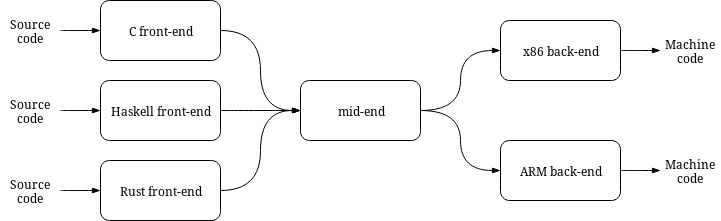
\includegraphics[width=11cm]{../background/llvm/figures/three_phase_compiler}
\end{frame}

\begin{frame}
	\frametitle{The Backend}

	\begin{itemize}
		\item instruction selection
		\item instruction scheduling
		\item register allocation
		\item code layout optimization
		\item assembly code emission
	\end{itemize}

\end{frame}

\begin{frame}
	\frametitle{LLVM Machine Specific Representation}

	\begin{itemize}
		\item	In-memory data structures
		\item	Can be serialized into \textit{Machine Intermediate Representation} (YAML).
	\end{itemize}

\end{frame}

\begin{frame}
	\frametitle{LLVM MIR}

	\lstinputlisting[language=C,tabsize=2,frame=single,breaklines=true,showstringspaces=false]
	{../background/llvm/examples/factorial.c}

\end{frame}


\begin{frame}
	\frametitle{LLVM MIR}

	\lstinputlisting[basicstyle=\tiny,tabsize=2,frame=single,breaklines=true,showstringspaces=false]
	{../background/llvm/examples/factorial.mir}

	Courtesy of the Unison documentation.
\end{frame}

\begin{frame}
	\frametitle{Problems}

	\begin{itemize}
		\item Treating each task a distinct steps
		\item Machine specific problems
	\end{itemize}
\end{frame}
